\graphicspath{{./images/}}      
\def\CHAPTERONE{./chapters/Chapter-1} 

\chapter{Experimente}
\label{chap:experiments}
%	\input{\CHAPTERONE /motivation}
\glsresetall
Im folgenden Kapitel werden die Experimente beschrieben, die im Rahmen dieser Arbeit durchgeführt wurden, um die Objekterkennung in fotorealistischen Bildern zu evaluieren. Für die Experimente wurden mit dem in Kapitel \ref{sec:takingpics} vorgestellten Verfahren 114 Szenen erstellt und von ihnen fünf Bilder aufgenommen. Jede Szene enthält zwischen 2 und 5 Objekten. Jedes Objekt ist einem oder mehreren folgender Szenarios zugeordnet: \textit{breakfast}, \textit{cooking} oder \textit{fridge}. Die Zuordnung ist in Tabelle \ref{tab:objects} einzusehen. Eine Szene enthält nur Objekte eines Szenarios. Dies ist echten Bedingungen nachempfunden, denn in der Regel finden sich im Kühlschrank keine Gabeln, Milch allerdings schon, die auch auf einem Frühstückstisch zu finden sein kann. Es wurden jeweils 50 \textit{breakfast} und \textit{cooking} Szenen und 14 \textit{fridge} Szenen erstellt. Insgesamt stehen so 570 Unreal-Bilder zur Verfügung. \par

In einem ersten Experiment wird ein \gls{klassifikator} trainiert und mit den Unreal-Bildern getestet. \todo{ausweiten?} 


\section{Klassifizierung über Merkmale}
\label{sec:classificationExperiment}
Die zuvor erstellten Unreal-Bilder, werden in einem ersten Experiment über Merkmale klassifiziert. Dazu wird ein Annotator aus dem \robosherlock-Paket \textit{rs\_addons} als \gls{klassifikator} mit echten Bildern der verwendeten Objekte trainiert. Mehr zu dem Paket und den \glspl{klassifikator} ist in \ref{sec:classifiers} auf Seite \pageref{sec:classifiers} zu finden. \par

Als \gls{klassifikator} wird der RFAnnotator benutzt, der auf einer \gls{rf} Implementierung basiert. Die zu unterscheidenden 20 Klassen sind in der Tabelle \ref{tab:objects} zu finden. Die Bilder der echten Objekte wurden den Klassen zugeordnet, bevor der \gls{klassifikator} damit trainiert wurde. Da es sich um einen Annotator für \robosherlock handelt, wurde eine \gls{ae} mit einigen \textit{hyotheses generators}, dem CaffeAnnotator zum Extrahieren der Merkmale (siehe Kap. \ref{sec:caffeAnno}, S.\pageref{sec:caffeAnno}), dem UnrealGTAnnotator zum herausziehen der \gls{gt} aus den Unreal-Bildern und dem \gls{klassifikator} erstellt. Um die Ergebnisse später verarbeiten zu können werden sie mit dem MLNInference (siehe Kap. \ref{sec:mlnInferencer}, S. \pageref{sec:mlnInferencer}) als logische Prädikate ausgegeben. \par
 
Die so erhaltene Klassifizierung für jedes Objekt wird mit der \gls{gt} verglichen, um so die Erkennungsrate des \gls{klassifikator}s zu ermitteln. Die Ergebnisse sind in Abbildung \ref{fig:classiRF_Ex_confMatrix} und Tabelle \ref{tab:classiRF_Ex_classMetrics} abgebildet. Während nahezu alle Objekte eine \gls{accuracy} über 90\% aufweisen, zeigen \gls{precision}, \gls{recall} und \gls{f1score}, dass der RFAnnotator große Schwierigkeiten hat, ähnliche Objekte auseinander zu halten. Besonders häufig werden Objekte fälschlicherweise als Milch (Milk) und Salz (TableSalt)  eingeordnet. Dies ist auf die box-artige Form und die Ähnlichkeit der Farbe vieler Objekte zu der Milch und dem Salz zurückzuführen, welche insgesamt in größerer Zahl in den Daten vorkommen als andere Objektklassen. Des weiteren hat der \gls{klassifikator} Schwierigkeiten das Geschirr auseinander zu halten, was auf die Größe dessen zurückzuführen ist. Besonders schlecht schneidet der Pfannenwender (Spatula) ab, der nicht einmal korrekt erkannt wurde. Mit einem \gls{f1score} über 0,8 schneiden die Objektklassen Buttermilch (Buttermilk), Kaffee (Coffee), Becher (Cup) und PancakeMix am besten ab. Diese Klassen unterscheiden sich in Form (Buttermilk, PancakeMix) und Farbe (Coffee, Cup) stark von den anderen Objekten.  

\begin{figure}
	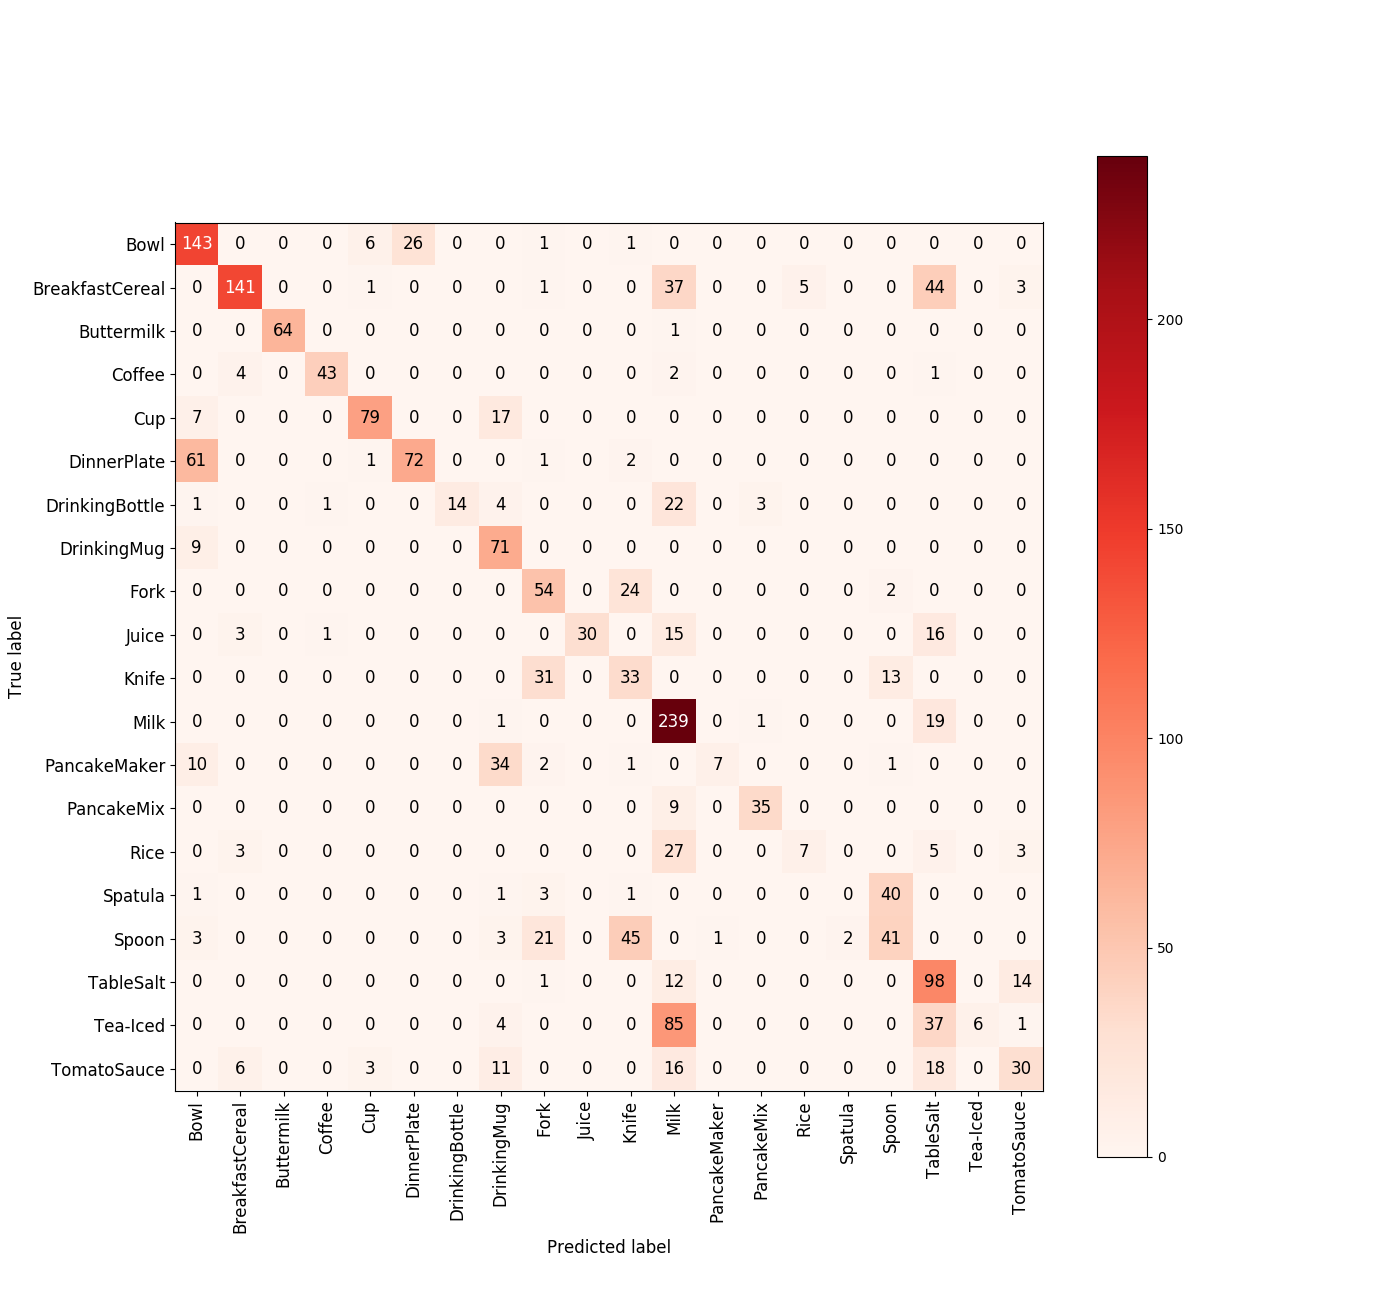
\includegraphics[scale=.4]{img/chapter6/classifierRFconf_matrix.png}
\caption[Konfusionsmatrix der Klassifizierung durch den RFAnnotators]{Die Konfusionsmatrix für die Klassifikation der Unreal-Bilder durch den mit echten Bildern trainierten RFAnnotator.}
\label{fig:classiRF_Ex_confMatrix}
\end{figure}

\begin{table}
\rowcolors{1}{}{lightgray}
\begin{tabularx}{\textwidth}{Xllll}
\textbf{Objekt}	& \textbf{\gls{accuracy}} & \textbf{\gls{precision}}	& \textbf{\gls{recall}}	& \textbf{\gls{f1score}} \\ \hline
Bowl & 0.91 & 0.61 & 0.81 & 0.69 \\  
BreakfastCereal & 0.92 & 0.9 & 0.61 & 0.72 \\  
Buttermilk & 1.0 & 1.0 & 0.98 & 0.99 \\  
Coffee & 0.99 & 0.96 & 0.86 & 0.91 \\  
Cup & 0.97 & 0.88 & 0.77 & 0.82 \\  
DinnerPlate & 0.93 & 0.73 & 0.53 & 0.61 \\  
DrinkingBottle & 0.97 & 1.0 & 0.31 & 0.47 \\  
DrinkingMug & 0.93 & 0.49 & 0.89 & 0.63 \\  
Fork & 0.93 & 0.47 & 0.68 & 0.55 \\  
Juice & 0.97 & 1.0 & 0.46 & 0.63 \\  
Knife & 0.91 & 0.31 & 0.43 & 0.36 \\  
Milk & 0.83 & 0.51 & 0.92 & 0.66 \\  
PancakeMaker & 0.96 & 0.88 & 0.13 & 0.22 \\  
PancakeMix & 0.99 & 0.9 & 0.8 & 0.84 \\  
Rice & 0.97 & 0.58 & 0.16 & 0.25 \\  
Spatula & 0.96 & 0.0 & 0.0 & 0.0 \\  
Spoon & 0.9 & 0.42 & 0.35 & 0.38 \\  
TableSalt & 0.88 & 0.41 & 0.78 & 0.54 \\  
Tea-Iced & 0.9 & 1.0 & 0.05 & 0.09 \\  
TomatoSauce & 0.94 & 0.59 & 0.36 & 0.44 \\  
\end{tabularx}
\caption[Objekt-spezifische Kenngrößen des RFAnnotators]{Kenngrößen für die einzelnen Objekte aus der Klassifizierung der Unreal-Bilder mit dem RFAnnotator.}
\label{tab:classiRF_Ex_classMetrics}
\end{table}

In einem zweiten Versuch wurde statt des RFAnnotators der SVMAnnotator verwendet, der auf einer \gls{svm} basiert. Die Ergebnisse sind in Abbildung  \ref{fig:classiSVM_Ex_confMatrix} zu sehen. Insgesamt sind die Ergebnisse gegenüber dem RFAnnotator etwas besser, da der SVMAnnotator mit 62\% eine etwas bessere \gls{accuracy} als der RFAnnotator mit 60\% aufweist. Jedoch werden vom SVMAnnotator neben dem Pfannenwender auch der PancakeMaker gar nicht richtig eingeordnet und auch die Flasche (DrinkingBottle) schneidet sehr schlecht ab. Der SVMAnnotator ist insgesamt bei einigen Klassen etwas zuverlässiger, hat jedoch auch einige große Fehlerquellen. 

\begin{figure}
	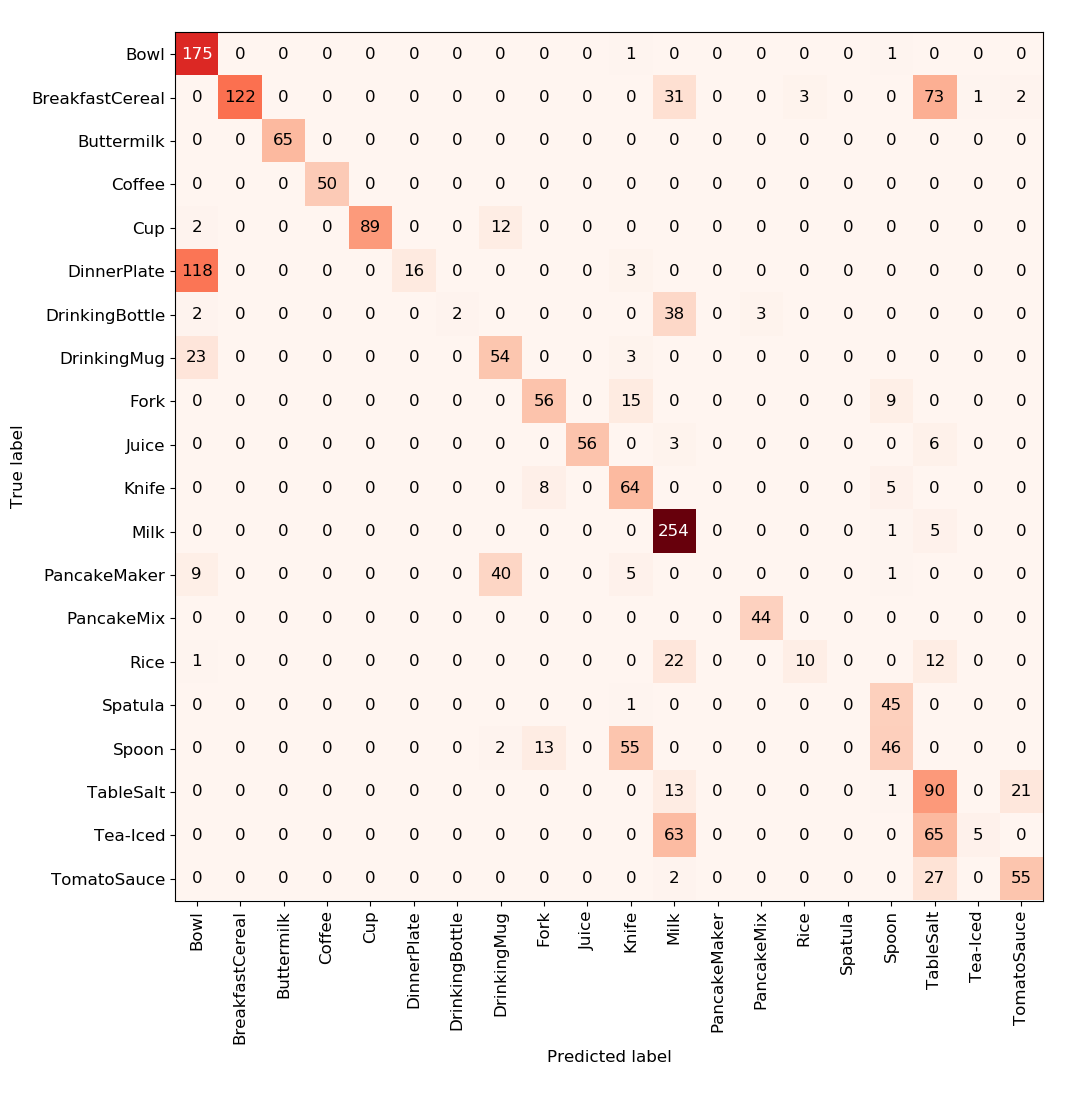
\includegraphics[scale=.4]{img/chapter6/classifierSVMconf_matrix.png}
\caption[Konfusionsmatrix der Klassifizierung durch den SVMAnnotators]{Die Konfusionsmatrix für die Klassifikation der Unreal-Bilder durch den mit echten Bildern trainierten SVMAnnotator.}
\label{fig:classiSVM_Ex_confMatrix}
\end{figure}

%\begin{table}
%\rowcolors{1}{}{lightgray}
%\begin{tabularx}{\textwidth}{Xllll}
%\textbf{Objekt}	& \textbf{\gls{accuracy}} & \textbf{\gls{precision}}	& \textbf{\gls{recall}}	& \textbf{\gls{f1score}} \\ \hline
%Bowl & 0.89 & 0.53 & 0.99 & 0.69 \\  
%BreakfastCereal & 0.92 & 1.0 & 0.53 & 0.69 \\  
%Buttermilk & 1.0 & 1.0 & 1.0 & 1.0 \\  
%Coffee & 1.0 & 1.0 & 1.0 & 1.0 \\  
%Cup & 0.99 & 1.0 & 0.86 & 0.93 \\  
%DinnerPlate & 0.91 & 1.0 & 0.12 & 0.21 \\  
%DrinkingBottle & 0.97 & 1.0 & 0.04 & 0.09 \\  
%DrinkingMug & 0.94 & 0.5 & 0.68 & 0.57 \\  
%Fork & 0.97 & 0.73 & 0.7 & 0.71 \\  
%Juice & 0.99 & 1.0 & 0.86 & 0.93 \\  
%Knife & 0.93 & 0.44 & 0.83 & 0.57 \\  
%Milk & 0.88 & 0.6 & 0.98 & 0.74 \\  
%PancakeMaker & 0.96 & 0.0 & 0.0 & 0.0 \\  
%PancakeMix & 1.0 & 0.94 & 1.0 & 0.97 \\  
%Rice & 0.97 & 0.77 & 0.22 & 0.34 \\  
%Spatula & 0.96 & 0.0 & 0.0 & 0.0 \\  
%Spoon & 0.9 & 0.42 & 0.4 & 0.41 \\  
%TableSalt & 0.85 & 0.32 & 0.72 & 0.45 \\  
%Tea-Iced & 0.91 & 0.83 & 0.04 & 0.07 \\  
%TomatoSauce & 0.96 & 0.71 & 0.65 & 0.68 \\  
%\end{tabularx}
%\caption[Objekt spezifische Kenngrößen des SVMAnnotators]{Kenngrößen für die einzelnen Objekte aus der Klassifizierung der Unreal-Bilder mit dem SVMAnnotator.}
%\label{tab:classiSVM_Ex_classMetrics}
%\end{table}

\section{Unreal-Bilder}
\label{sec:onlyUnrealImages}
Im folgenden Experiment werden nur Unreal-Bilder zum trainieren und testen des \gls{mlns} verwendet. Als \gls{gt} dienen die Objektklassen. Die logischen Prädikate wurden dazu mit der in Kapitel \ref{sec:analysisengine} vorgestellten \gls{ae} aus den 570 Unreal-Bildern extrahiert. Diese werden wie in Tabelle \ref{tab:annotators} auf S.\pageref{tab:annotators} beschrieben für das Modell deklariert.  Zusätzlich gibt es noch das $scene$-Prädikat und eine Einschränkung für das $object$-Prädikat:
\begin{itemize}
\item das $scene(scene)$ Prädikat ordnet die Szene in einen räumlichen Kontext ein. Die Domäne für das Prädikat ist $dom(scene) = \{breakfast, cooking, fridge\}$
\item das Prädikat $object$ wird folgendermaßen definiert: $object(cluster, object!)$. Der \glqq!\grqq \ Operator besagt, dass dieses Prädikat als funktionelle Einschränkung behandelt werden soll. Das bedeutet, dass immer exakt ein Atom wahr sein muss; alle anderen sind falsch.\footnote{\url{http://pracmln.org/mln_syntax.html}} Im Falle des obigen Prädikats bedeutet das, dass jedem Cluster genau eine Objektklasse zugeordnet sein muss. Dies macht im Rahmen des Modells Sinn, da ein Objekt nicht mehreren Klassen zugleich angehören kann und wurde auch von Nyga et al.\cite{pr2looking} in ihrer \gls{mln}-Deklaration angenommen.
\end{itemize}
Das Folgende \gls{mln} beschreibt die Zusammenhänge der einzelnen Informationen der Annotatoren und der Objektklassen:
\begin{align*}
& w_{1} \ shape(?c, +?sha) \wedge object(?c, +?obj) \\
& w_{2} \ color(?c, +?col) \wedge object(?c, +?obj) \\
& w_{3} \ size(?c, +?size) \wedge object(?c, +?obj) \\
& w_{4} \ instance(?c, +?inst) \wedge object(?c, +?obj) \\
& w_{5} \ goggles\_Logo(?c, +?comp) \wedge object(?c, +?obj)\\
& w_{6} \ goggles\_Text(?c, +?text) \wedge object(?c, +?obj)\\
& w_{7} \ goggles\_Product(?c, +?prod) \wedge object(?c, +?obj)\\
& w_{8} \ scene(+?s) \wedge object(?c, +?obj)\\
& w_{9} \ object(?c1, +?t1) \wedge object(?c2, +?t2) \wedge ?c1 =/= ?c2
\end{align*}
\textit{Hinweise zur Syntax von \pracmln:} Jeder Variable muss ein \glqq ?\grqq \ vorangestellt werden. Das \glqq +\grqq \ bedeutet, dass für jedes Element der Domäne dieser Variable eine Formel erstellt wird. \footnote{\url{http://pracmln.org/mln_syntax.html}}  \par
 
Ein \gls{mln} wurde mit \textit{Discriminative Pseudo-likelihood Learning with Custom Grounding}   trainiert. Es wurde die \textit{Discrimitive} Variante des Lernalgorithmus gewählt, da es ein genaueres Modell und geringeren Rechenaufwand bietet. Als Voraussetzung müssen bestimmte Prädikate bei den Anfragen entweder nur in den Anfragen oder der Evidenzen vorkommen. Da in diesem Fall die Objektklasse erkannt werden soll, ist das $object$-Prädikat die einzige Anfrage and das trainierte \gls{mln}. Die \textit{Custom Grounding} Variante bietet eine schnellere Rechenzeit, wenn die Formeln größtenteils aus Konjunktionen bestehen. Eine Regularisierung findet durch den Gaussian-Prior mit einem Mittelwert $\mu = 0$ und einer Standardabweichung $\sigma = 10$ statt. \par   

Zum Testen werden Anfragen, um welche Objekte es sich bei den Clustern handelt, an das trainierte \gls{mln} gestellt. Es soll also die bedingte Wahrscheinlichkeit $P(object \mid E)$ berechnet werden. Es wird eine Evidenz angegeben, die von der Form her den Trainingsdaten entspricht, also eine wahrgenommene Szene darstellt, nur ohne das $object$-Prädikat, da die Objektklasse sonst schon bekannt wäre und nicht aus den anderen Eigenschaften darauf geschlossen werden muss. Als Inferenzmechanismus wird \textit{WCSP} verwendet. Dies ist ein Algorithmus, der die \textit{Most Probable Explanation (MPE)} berechnet, also nicht die gesamte bedingte Wahrscheinlichkeit, sondern nur die wahrscheinlichste Variablenbelegung unter Bedingung der Evidenz. WCSP wandelt das instanziierte \gls{mn} dazu in ein \textit{gewichtetes Constraint Satisfaction Problem} um. \par

Um dieses Modell zu evaluieren, wird 10-fache Kreuzvalidierung durchgeführt. Dabei wird der gesamte Datensatz, also alle 570 Bilder, in 10 Teilmengen aufgeteilt. Jedes Bild bleibt für den gesamten Prozess in seiner Teilmenge. Nun werden 9 Teilmengen als Trainingsdaten für ein \gls{mln} benutzt, während die übrige 10. Teilmenge zum Testen zur Verfügung steht. Dieser Vorgang wird 10 mal durchgeführt, sodass jede Teilmenge genau einmal zum Testen verwendet wurde. Die Ergebnisse der einzelnen Durchgänge können nun gemittelt werden. Dies verhindert Überanpassung des Modells, also die Anpassung an die Trainingsdaten und damit einen Verlust der Generalität des Modells. \par

Die Ergebnisse der Kreuzvalidierung sind in Abbildung \ref{fig:unreal_1_confMatrix} und Tabelle \ref{tab:unreal_1_classMetrics} dargestellt. Insgesamt werden eine hohe \gls{accuracy} für alle Objektklassen als auch Werte über 90\% für \gls{precision}, \gls{recall} und \gls{f1score} erreicht. Einzig das Besteck und der Reis schneiden etwas schlechter ab. Bei dem Besteck war dies erwartet, da Messer, Gabeln und Löffeln kleiner sind als viele andere Objekte und damit visuelle Eigenschaften schwieriger auszumachen sind. Im Gegensatz zu den Ergebnissen der \glspl{klassifikator} ist eine deutliche Verbesserung zu erkennen. Vor allem gibt es keine Objekte, die gar nicht erkannt werden. Die bessere Erkennungsrate war jedoch erwartet, da \glspl{mln} die Ergebnisse verschiedener Experten, also Annotatoren in \robosherlock, kombiniert und solche Ensembles, wie bereits zuvor dargelegt, zu besseren Ergebnissen kommen können. \newline
In den Abbildungen \ref{fig:singleEvidences} und \ref{fig:singleEvidencesGog} sind die Ergebnisse der Erkennung mit nur jeweils einer Evidenz, also einem logischen Prädikat, abgebildet. Es ist zu erkennen, dass bei Farbe, Form und Größe einige bestimmte Objekte bei der entsprechenden Evidenz präferiert werden. Bei der Instanz fällt auf, dass vieles als PancakeMaker eingeordnet wird, während viele Objekt auch richtig zugeordnet sind, was auf eine schlechte Performance des entsprechenden \gls{klassifikator}s hinweist. Der \texttt{GogglesAnnotator} annotiert vor allem texturierte Objekte, jedoch auch einige andere, welche er dann auch selten wiedererkennt. Insgesamt unterstützen diese Ergebnisse die Idee einer besseren Erkennung durch Ensembles, da jeder Annotator seine stärken und Schwächen aufweist, und erst durch die Zusammenführung der einzelnen Ergebnisse eine gute Erkennungsrate erreicht wird.

\begin{figure}
	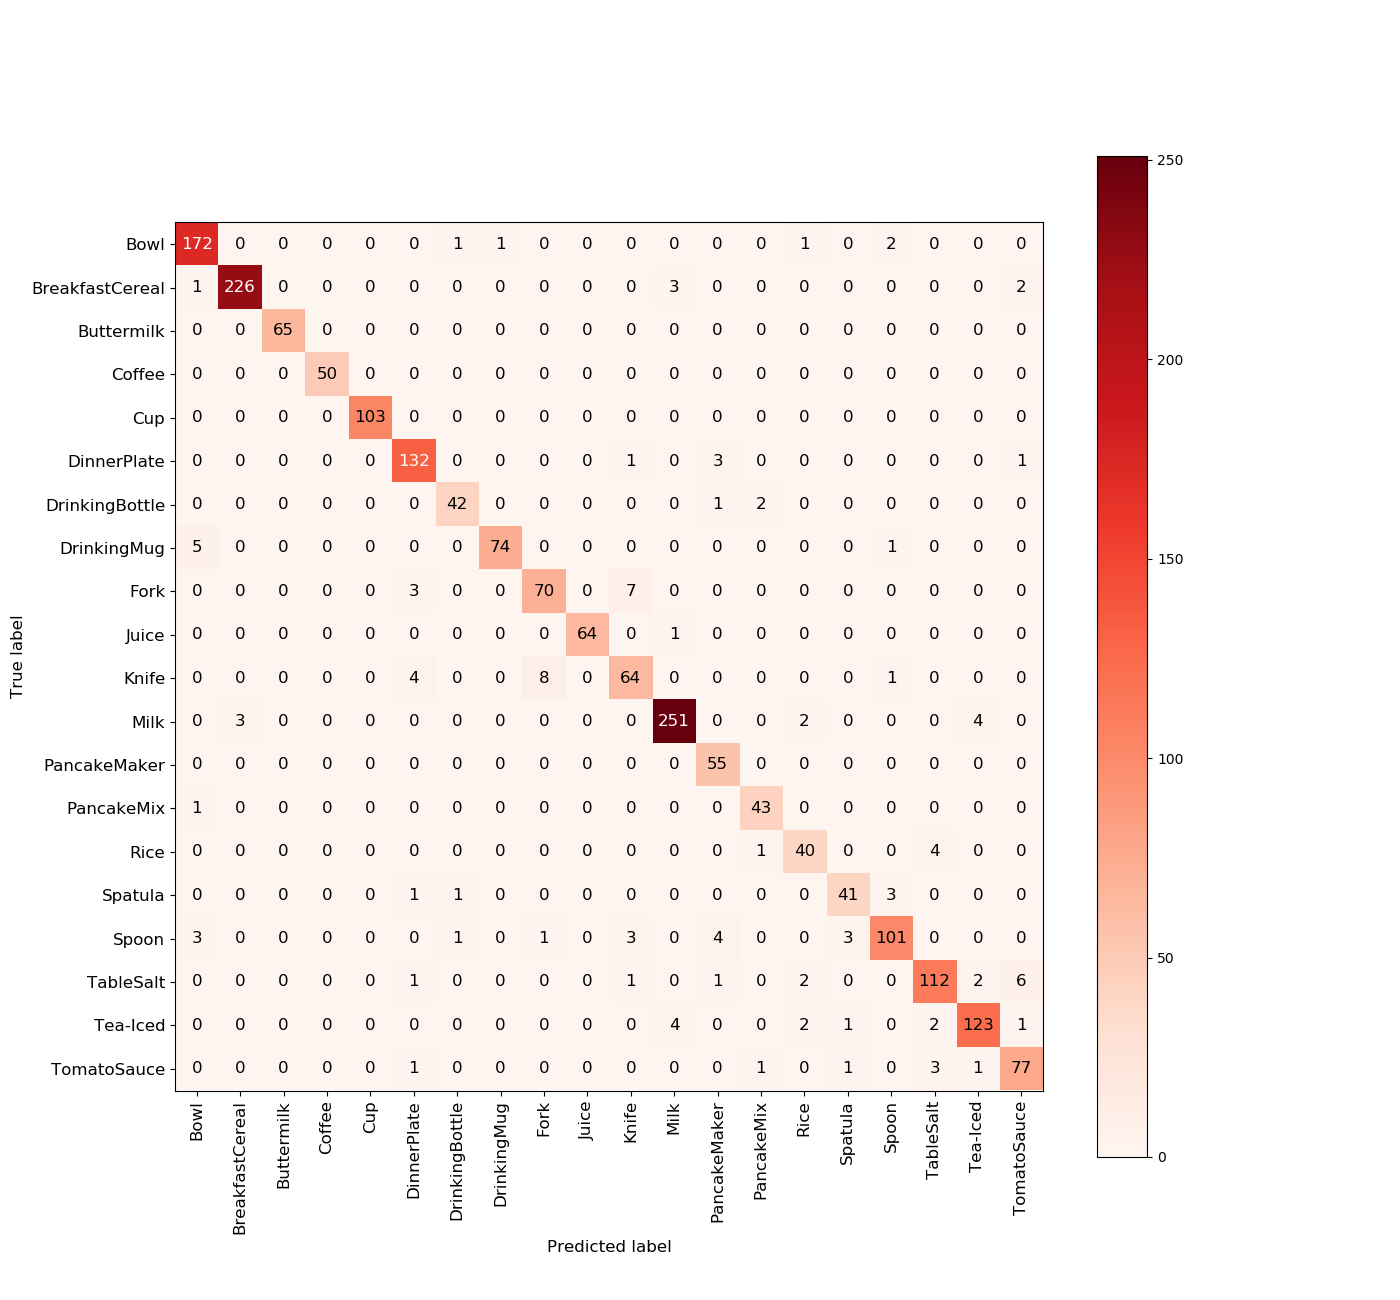
\includegraphics[scale=.5]{img/chapter6/unrealEx1_cof_matrix.png}
\caption[Konfusionsmatrix des gesamten Unreal-Bilder Datensatzes]{Die Konfusionsmatrix für die 10-fache Kreuzvalidierung der gesamten 570 Unreal-Bilder.}
\label{fig:unreal_1_confMatrix}
\end{figure}

\begin{table}
\rowcolors{1}{}{lightgray}
\begin{tabularx}{\textwidth}{Xllll}
\textbf{Objekt}	& \textbf{\gls{accuracy}} & \textbf{\gls{precision}}	& \textbf{\gls{recall}}	& \textbf{\gls{f1score}} \\ \hline
Bowl & 0.99 & 0.95 & 0.98 & 0.97 \\  
BreakfastCereal & 1.0 & 1.0 & 0.98 & 0.99 \\  
Buttermilk & 1.0 & 1.0 & 1.0 & 1.0 \\  
Coffee & 1.0 & 1.0 & 1.0 & 1.0 \\  
Cup & 1.0 & 1.0 & 1.0 & 1.0 \\  
DinnerPlate & 0.99 & 0.95 & 0.95 & 0.95 \\  
DrinkingBottle & 1.0 & 0.89 & 0.91 & 0.9 \\  
DrinkingMug & 0.99 & 0.97 & 0.9 & 0.94 \\  
Fork & 0.99 & 0.89 & 0.89 & 0.89 \\  
Juice & 1.0 & 1.0 & 0.98 & 0.99 \\  
Knife & 0.99 & 0.86 & 0.87 & 0.86 \\  
Milk & 0.99 & 0.97 & 0.98 & 0.98 \\  
PancakeMaker & 0.99 & 0.83 & 1.0 & 0.91 \\  
PancakeMix & 1.0 & 0.91 & 0.93 & 0.92 \\  
Rice & 0.99 & 0.87 & 0.91 & 0.89 \\  
Spatula & 1.0 & 0.91 & 0.91 & 0.91 \\  
Spoon & 0.99 & 0.94 & 0.89 & 0.92 \\  
TableSalt & 0.99 & 0.94 & 0.9 & 0.92 \\  
Tea-Iced & 0.99 & 0.98 & 0.95 & 0.96 \\  
TomatoSauce & 0.99 & 0.91 & 0.92 & 0.91 \\  
\end{tabularx}
\caption[Objekt-spezifische Kenngrößen des gesamten Unreal-Bilder Datensatzes]{Kenngrößen für die einzelnen Objekte aus der 10-fachen Kreuzvalidierung der gesamten Unreal-Bilder.}
\label{tab:unreal_1_classMetrics}
\end{table}


\begin{figure}
\centering
	\begin{subfigure}[b]{0.48\textwidth}
		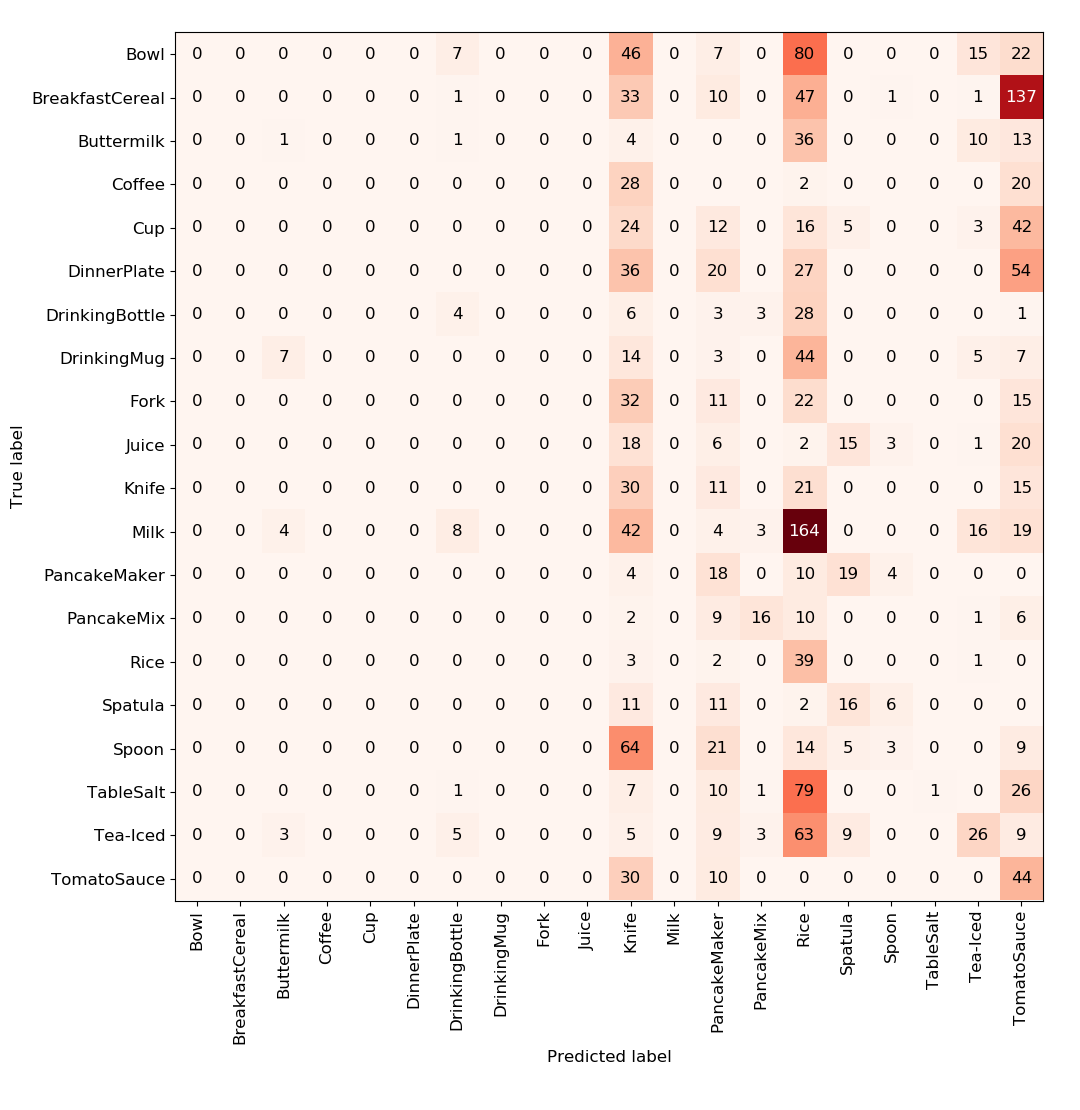
\includegraphics[scale=.27]{img/chapter6/unrealEx1_color}
		\subcaption{Farbe}
	\end{subfigure}
	\begin{subfigure}[b]{0.48\textwidth}
		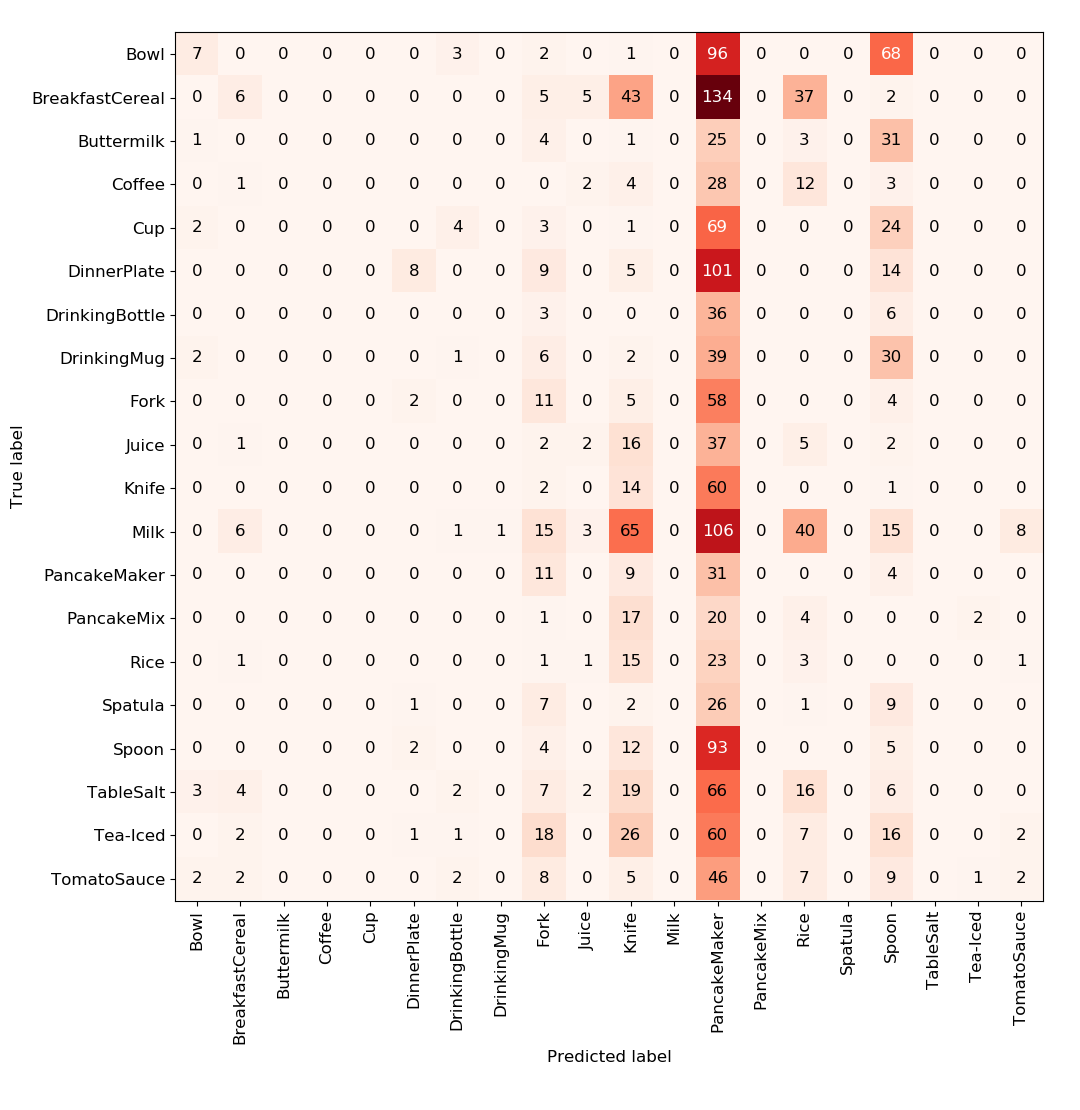
\includegraphics[scale=.27]{img/chapter6/unrealEx1_shape}	
		\subcaption{Form}
	\end{subfigure}
	\begin{subfigure}[b]{0.48\textwidth}
		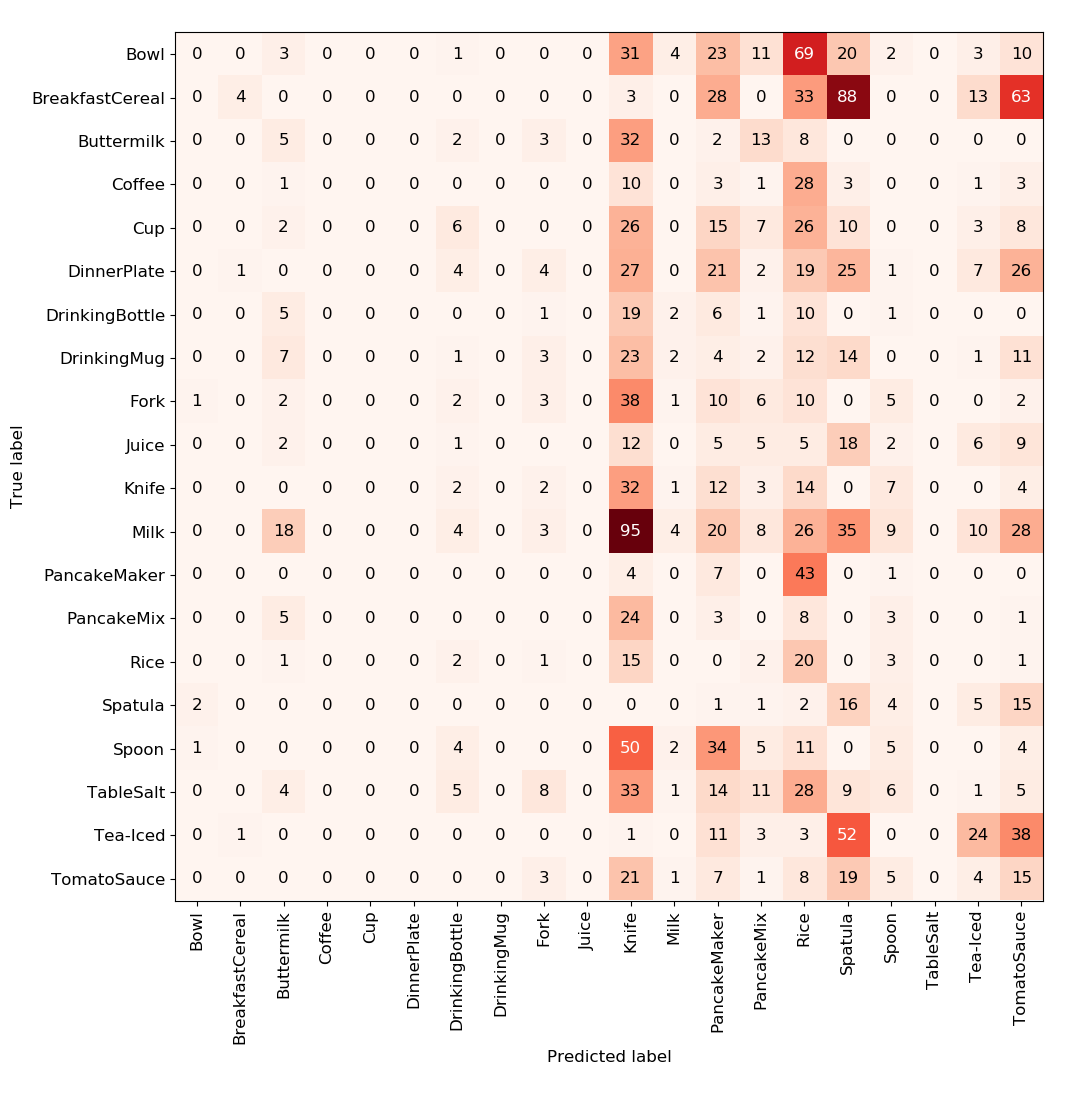
\includegraphics[scale=.27]{img/chapter6/unrealEx1_size}	
		\subcaption{Größe}
	\end{subfigure}
	\begin{subfigure}[b]{0.48\textwidth}
		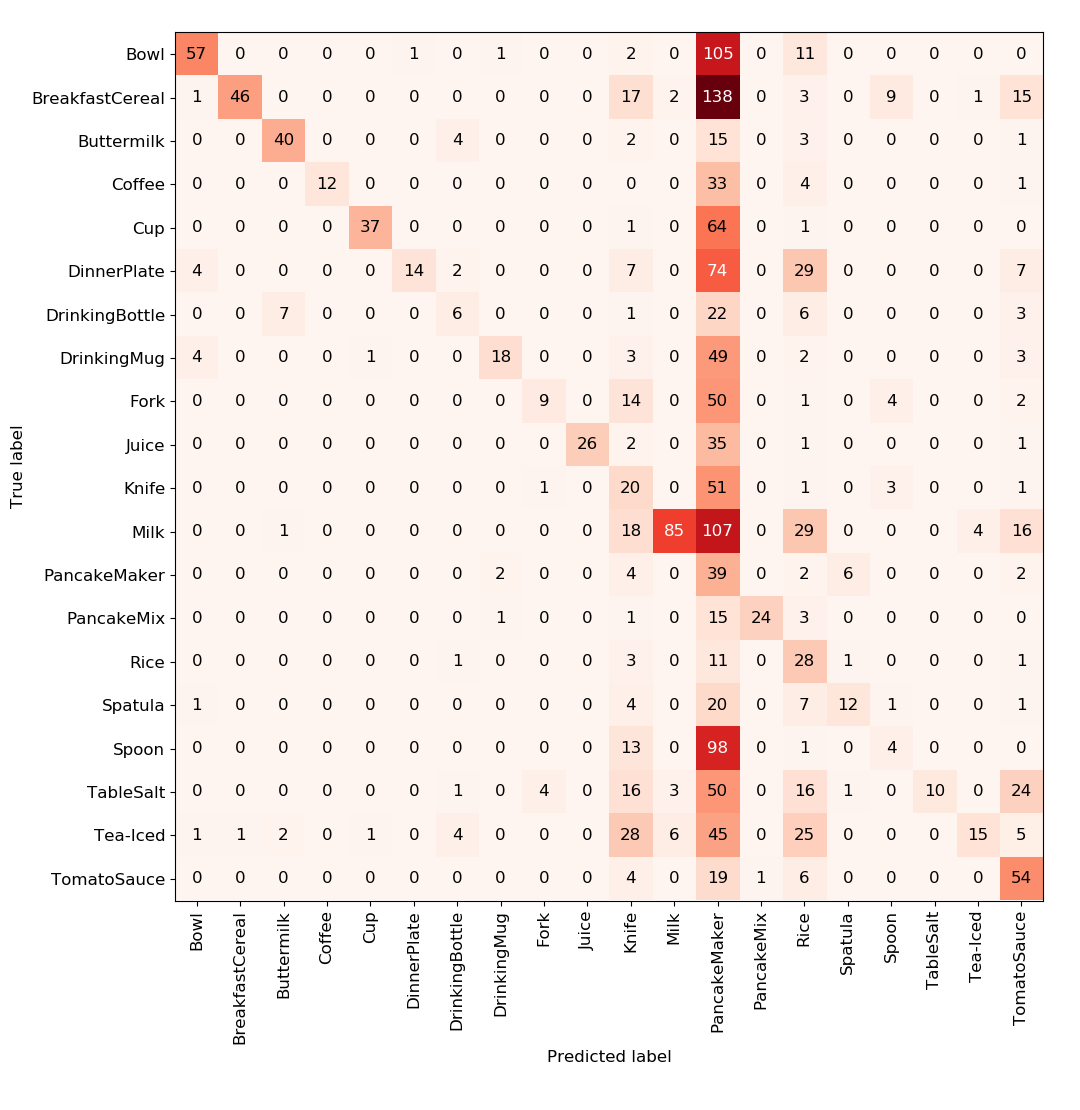
\includegraphics[scale=.27]{img/chapter6/unrealEx1_instance}	
		\subcaption{Instanz}
	\end{subfigure}
\caption[Konfusionsmatrizen für die Klassifikation mit Evidenz von nur einem Experten]{Konfusionsmatrizen für die 10-fache Kreuzvalidierung mit Evidenz von nur jeweils einem Experten.}
\label{fig:singleEvidences}
\end{figure}

\begin{figure}
	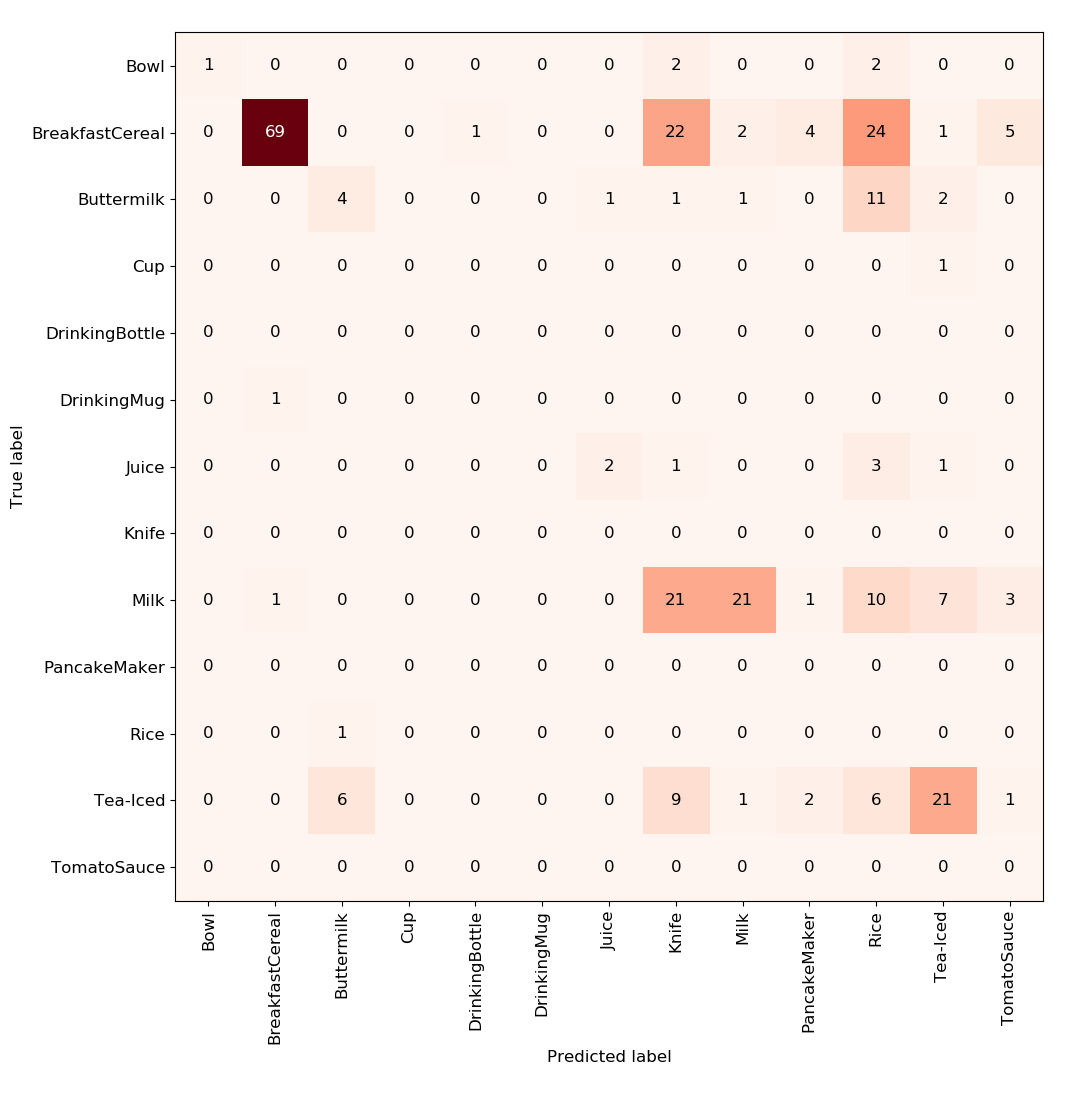
\includegraphics[scale=.27]{img/chapter6/unrealEx1_goggles}	
\caption[Konfusionsmatrix für die Klassifikation nur durch den \texttt{GogglesAnnotator}]{Konfusionsmatrix für die 10-fache Kreuzvalidierung nur durch den \texttt{GogglesAnnotator}}
\label{fig:singleEvidencesGog}
\end{figure}

\section{Reale Bilder als Testdaten}

Im folgenden Experiment werden reale Bilder als Testdaten verwendet. Dazu wurden mit dem PR2-Roboter des \gls{iai} Bilder in der realen Küchenumgebung aufgenommen. Die verwendeten Objekte sind dabei die echten Gegenstücke zu den eingescannten Objekten. Unglücklicherweise stand zu dem Zeitpunkt der Aufnahme der LinuxCup und die YellowPlate nicht mehr zur Verfügung. Für die YellowPlate wurde stattdessen ein weißer Teller als Ersatz Objekt verwendet. Es wurden wieder 114 zufällig aufgebaute Szenen mit der gleichen Szenarien-Verteilung erstellt. Die Bedingungen für das gemeinsame Auftreten von Objekten innerhalb der Szenarien bleibt ebenfalls gleich. Auf Grund des erhöhten Aufwandes bei der Aufnahme der Szenen, wurden von jeder Szene nur drei Bilder aufgenommen, womit insgesamt 342 reale Bilder zur Verfügung stehen. Im Gegensatz zu den Unreal-Bildern sind die Blickwinkel nicht exakt die Gleichen für jede Szene, da der Roboter bei der Aufnahme manuell bewegt werden muss (eine Szene ist in Abbildung \ref{fig:exampleSceneReal} zu sehen). Die Bilder wurden von der in Kapitel \ref{sec:analysisengine} beschriebenen \gls{ae} annotiert, allerdings ohne den \texttt{UnrealGTAnnotator} zu verwenden, da dieser nur für Bilder aus der \unreal geeignet ist, da echte Bilder keine Asset-Namen zur Bestimmung der \gls{gt} aufweisen. Dementsprechend wurde die \gls{gt} manuell annotiert.

\begin{figure}
\centering
	\begin{subfigure}[b]{0.3\textwidth}
		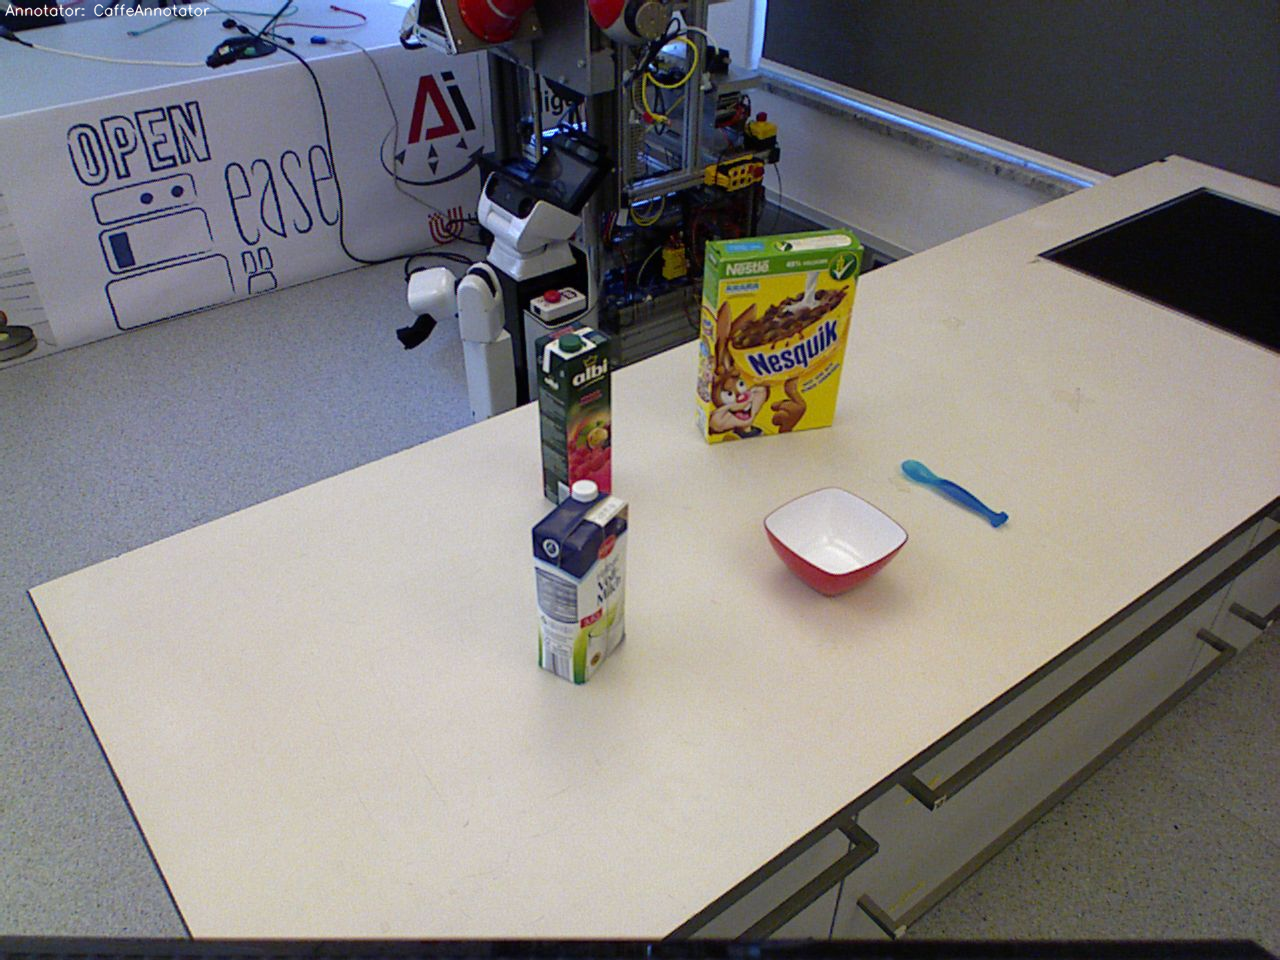
\includegraphics[scale=.1]{img/chapter6/real1}
	\end{subfigure}
	\quad
	\begin{subfigure}[b]{0.3\textwidth}
		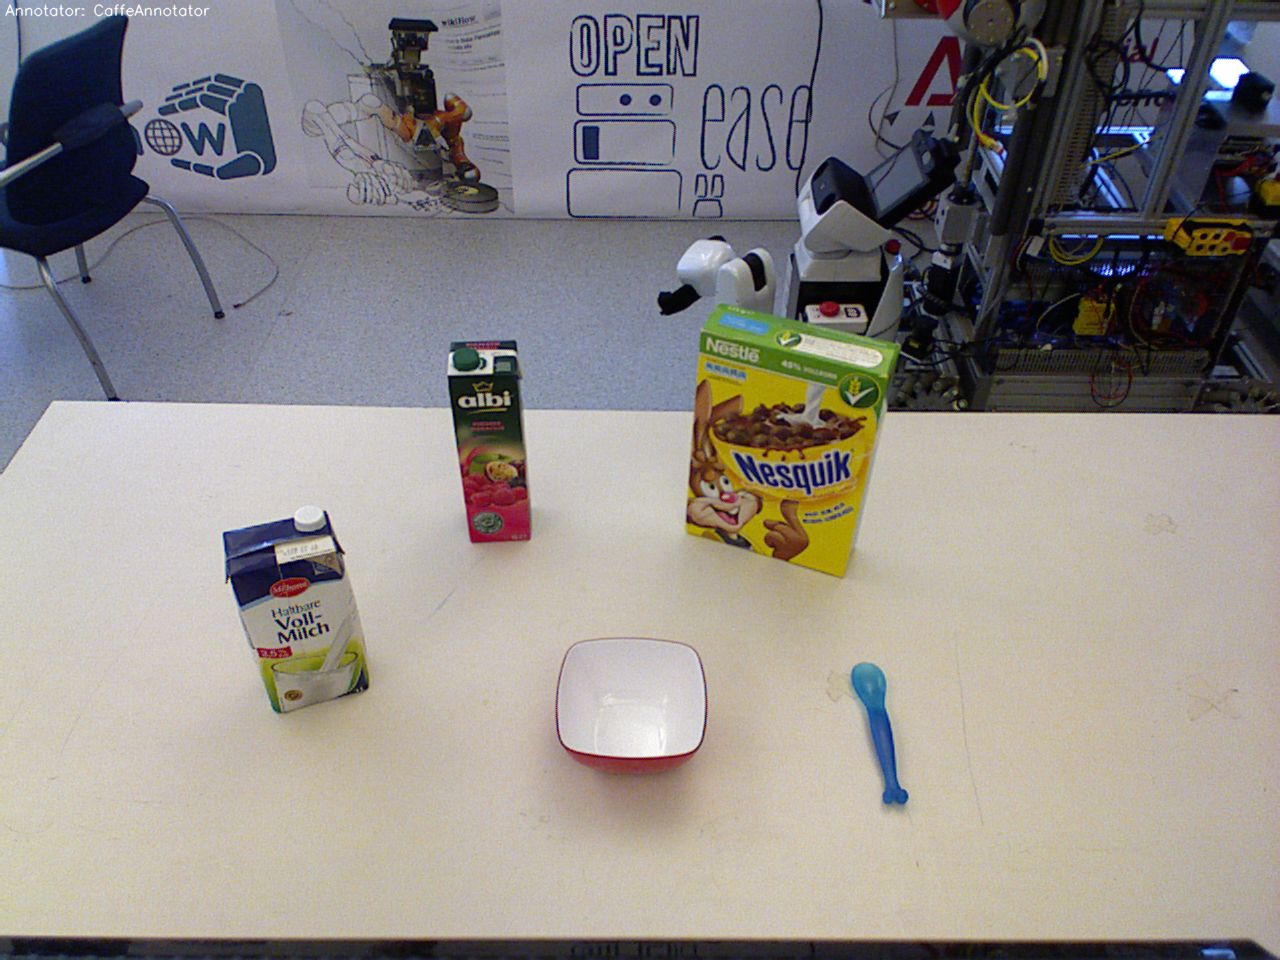
\includegraphics[scale=.1]{img/chapter6/real2}	
	\end{subfigure}
	\quad
	\begin{subfigure}[b]{0.3\textwidth}
		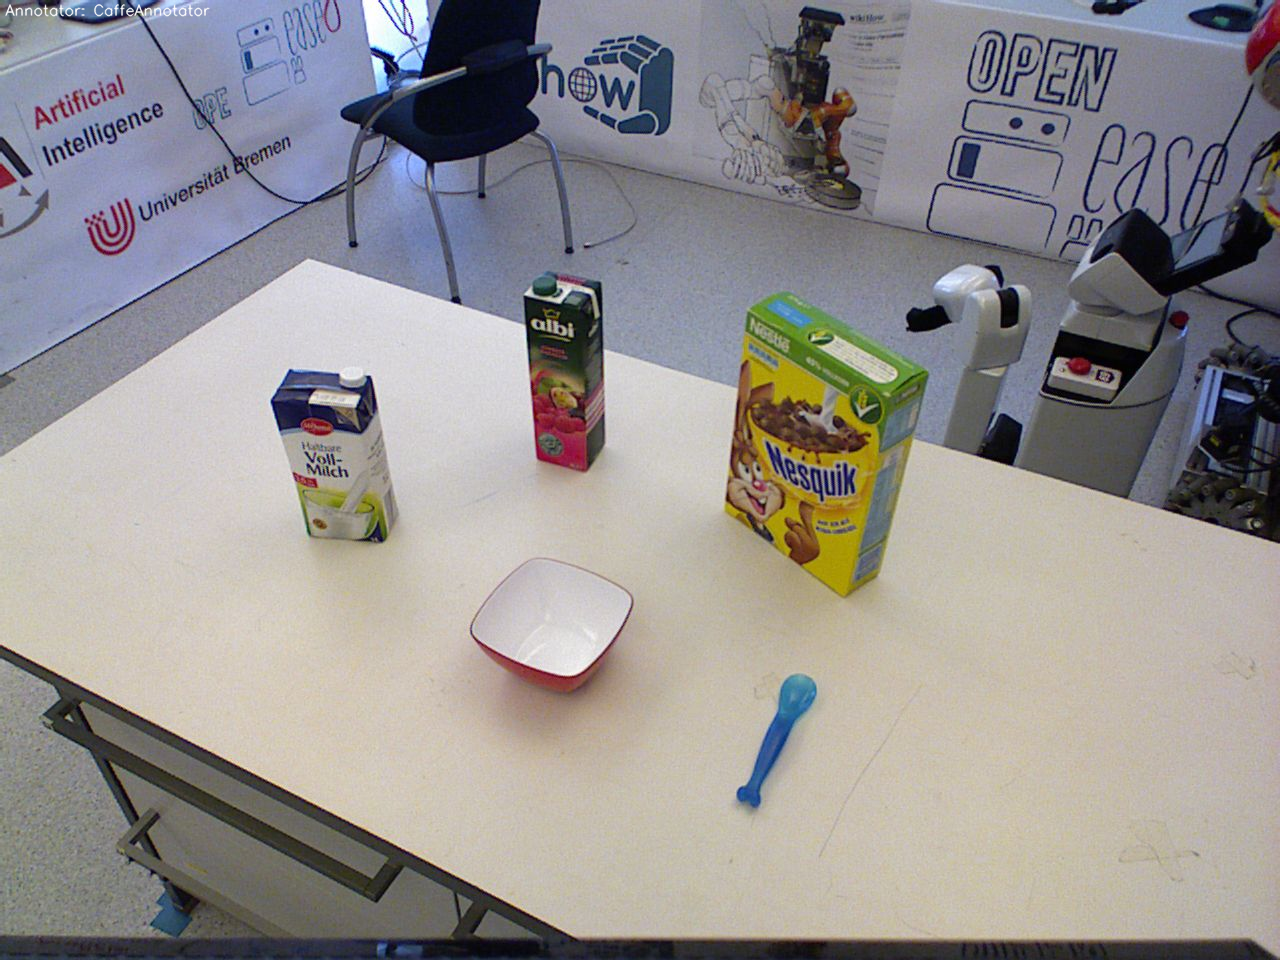
\includegraphics[scale=.1]{img/chapter6/real3}	
	\end{subfigure}
\caption[Reale Bilder einer Szene]{Ein Bildersatz der realen Szenen.}
\label{fig:exampleSceneReal}
\end{figure}

Es wurde nun ein \gls{mln} mit allen 570 Unreal-Bildern trainiert. Damit die Atome für den \texttt{GogglesAnnotator} in beiden Datensätzen übereinstimmen, wurde das Clustering mit den Annotationen aus beiden Datensätzen durchgeführt. Die Deklaration des \gls{mln} und Parameter beim Lernen sind unverändert wie im vorherigen Experiment, bei dem nur Unreal-Bilder zum Einsatz kamen. Die Bedingungen und Parameter für die Anfragen sind ebenfalls gleich \par

Die \gls{accuracy} ist für alle Klassen über 90\%, während auch die Werte für \gls{precision}, \gls{recall} und \gls{f1score} in den meisten Fällen mit über 70\% relativ hoch ausfallen. Ausnahmen bilden wie erwartet das Geschirr, aber auch die Trinkflasche, PancakeMix und Maker und der Reis. Interessanterweise schneiden Löffel und Gabeln dabei deutlich besser ab als Messer. Besonders schlecht schneidet auch der Pfannenwender ab, was auch schon bei den \glspl{klassifikator} aufgefallen ist. Da die 10-fache Kreuzvalidierung, bei der nur Unreal-Bilder verwendet wurden, dieses Problem nicht zeigt, kann angenommen werden, dass das 3D-Modell keine gute Repräsentation des echten Objektes ist. Dass die Performance bei Reis so stark abfällt, ist interessant, da die Erkennungsrate für andere texturierte Objekte (Müsli, Milch, Salz, Eistee, Tomaten Sauce) zwar auch sinkt, jedoch nicht so stark, wie beim Reis. Der wahrscheinlich wegen seiner Form von den \glspl{klassifikator} noch gut erkannte PancakeMix, scheint diesen Vorteil hier nicht ausspielen zu können, während das für die Buttermilch mit einer 100 prozentigen Erkennungsrate nicht gilt. Für den PancakeMaker scheint das Selbe zu gelten, wie für den Pfannenwender, da auch er schon bei den \glspl{klassifikator} eine Problemquelle war. 

\begin{figure}
	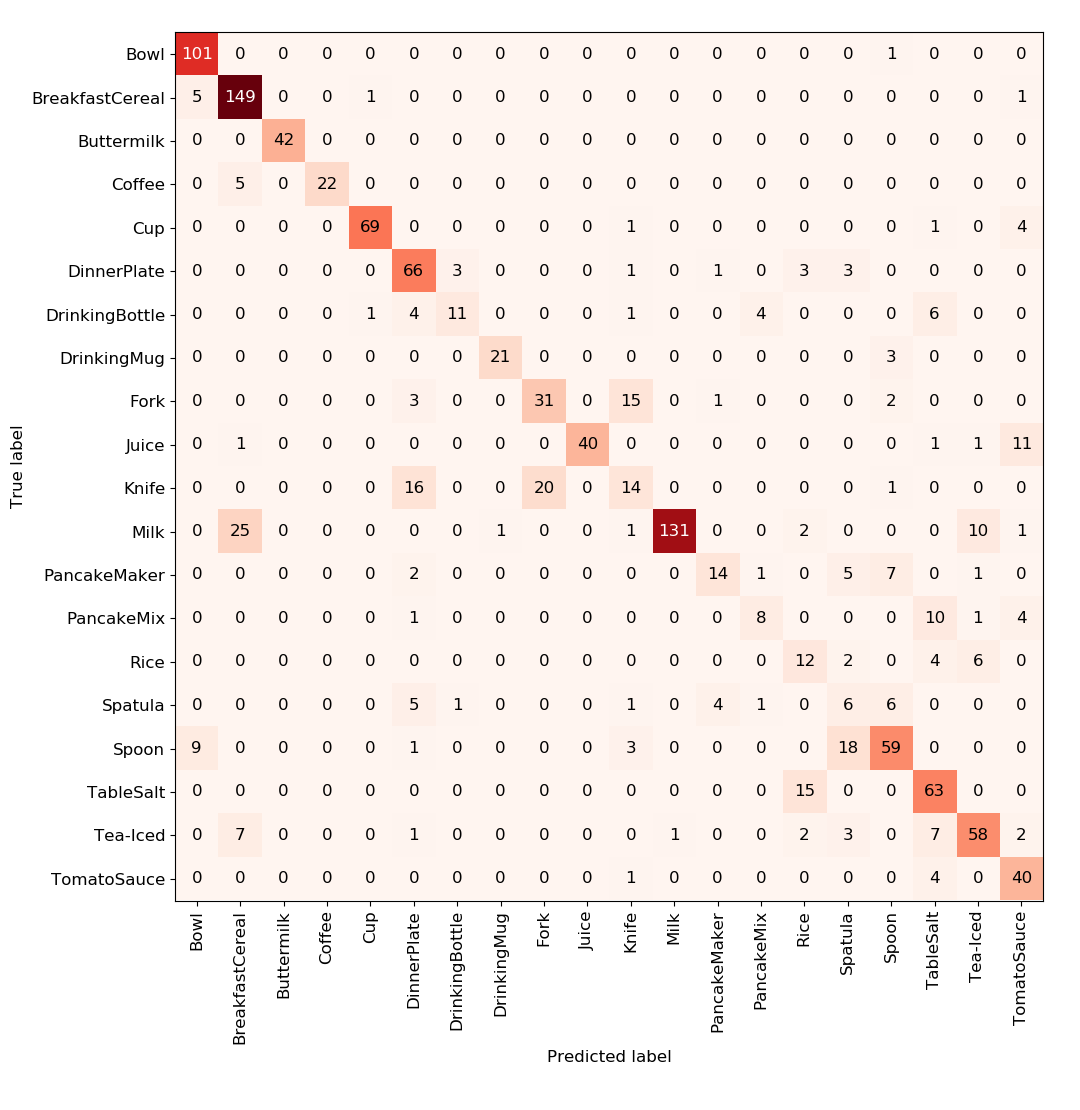
\includegraphics[scale=.4]{img/chapter6/unrealReal_conf_matrix}
\caption[Konfusionsmatrix der Klassifikation mit Unreal-Trainingsset und Real-Testset]{Die Konfusionsmatrix für die Klassifikation aller realen Bilder durch ein \gls{mln}, das mit allen Unreal-Bildern trainiert wurde.}
\label{fig:unrealRealconfMatrix}
\end{figure}  

\begin{table}
\rowcolors{1}{}{lightgray}
\begin{tabularx}{\textwidth}{Xllll}
\textbf{Objekt}	& \textbf{\gls{accuracy}} & \textbf{\gls{precision}}	& \textbf{\gls{recall}}	& \textbf{\gls{f1score}} \\ \hline
Bowl & 0.98 & 0.88 & 0.99 & 0.93 \\  
BreakfastCereal & 0.96 & 0.8 & 0.96 & 0.87 \\  
Buttermilk & 1.0 & 1.0 & 1.0 & 1.0 \\  
Coffee & 0.99 & 1.0 & 0.81 & 0.9 \\  
Cup & 0.99 & 0.97 & 0.92 & 0.95 \\  
DinnerPlate & 0.96 & 0.67 & 0.86 & 0.75 \\  
DrinkingBottle & 0.98 & 0.73 & 0.41 & 0.52 \\  
DrinkingMug & 1.0 & 0.95 & 0.88 & 0.91 \\  
Fork & 0.96 & 0.61 & 0.6 & 0.6 \\  
Juice & 0.99 & 1.0 & 0.74 & 0.85 \\  
Knife & 0.94 & 0.37 & 0.27 & 0.31 \\  
Milk & 0.96 & 0.99 & 0.77 & 0.86 \\  
PancakeMaker & 0.98 & 0.7 & 0.47 & 0.56 \\  
PancakeMix & 0.98 & 0.57 & 0.33 & 0.42 \\  
Rice & 0.97 & 0.35 & 0.5 & 0.41 \\  
Spatula & 0.95 & 0.16 & 0.25 & 0.2 \\  
Spoon & 0.95 & 0.75 & 0.66 & 0.7 \\  
TableSalt & 0.95 & 0.66 & 0.81 & 0.72 \\  
Tea-Iced & 0.96 & 0.75 & 0.72 & 0.73 \\  
TomatoSauce & 0.97 & 0.63 & 0.89 & 0.74 \\  
\end{tabularx}
\caption[Objekt-spezifische Kenngrößen der Klassifikation mit Unreal-Trainingsset und Real-Testset]{Kenngrößen für die einzelnen Objekte der Klassifikation der realen Bilder durch ein \gls{mln}, das mit allen Unreal-Bildern trainiert wurde.}
\label{tab:unreal_1_classMetrics}
\end{table}